\documentclass[11pt]{article}

\newcommand{\inv}{{-1}}
\newcommand{\numberthis}{\addtocounter{equation}{1}\tag{\theequation}}

\RequirePackage[l2tabu, orthodox]{nag}
%\documentclass{article}

\usepackage[left=1.in, right=1.in, top=1.25in, bottom=1.25in]{geometry}

% FONTS
\usepackage[T1]{fontenc}

% Replace default Latin Modern typewriter with its proportional counterpart
% http://www.tug.dk/FontCatalogue/lmoderntypewriterprop/
\renewcommand*\ttdefault{lmvtt}


%%% OPTION 1 - Fourier Math + New Century Schoolbook + ParaType Sans

% % Import Fourier Math (this imposes its own New Century Schoolbook type)
% % http://www.ctan.org/tex-archive/fonts/fouriernc/
%\usepackage{fouriernc}
%\usepackage{amsmath}
% % Replace with TeX Gyre Schola version of New Century Schoolbook (must scale!)
% % http://www.tug.dk/FontCatalogue/tgschola/
% \usepackage[scale=0.92]{tgschola}
% \usepackage[scaled=0.88]{PTSans}

%% OPTION 2 - MathDesign Math + Bitstream Charter + ParaType Sans

% Import MathDesign (this brings along Bitstream Charter)
% http://www.ctan.org/tex-archive/fonts/mathdesign/
\usepackage[bitstream-charter]{mathdesign}
\usepackage{amsmath}
\usepackage[scaled=0.92]{PTSans}


% %%% OPTION 3 - MTPRO 2 Math + Termes Times + ParaType Sans

% \usepackage{tgtermes}
% \usepackage{amsmath}
% \usepackage[subscriptcorrection,
%             amssymbols,
%             mtpbb,
%             mtpcal,
%             nofontinfo  % suppresses all warnings
%            ]{mtpro2}
% \usepackage{scalefnt,letltxmacro}
% \LetLtxMacro{\oldtextsc}{\textsc}
% \renewcommand{\textsc}[1]{\oldtextsc{\scalefont{1.10}#1}}
% \usepackage[scaled=0.92]{PTSans}

% Use default fonts here
% \usepackage{amsmath}
% \usepackage{amssymb}

\usepackage{titling}

% COLOR
\usepackage[table,usenames,dvipsnames]{xcolor}
\definecolor{shadecolor}{gray}{0.9}

% SPACING and TEXT
\usepackage[final,expansion=alltext]{microtype}
\usepackage[english]{babel}
\usepackage[parfill]{parskip}
\usepackage{afterpage}
\usepackage{framed}
\usepackage{verbatim}
\usepackage{setspace}

%redefine the leftbar environment to accept a width and coloring options
\renewenvironment{leftbar}[1][\hsize]
{%
  \def\FrameCommand
  {%
    {\color{Gray}\vrule width 3pt}%
    \hspace{10pt}%
    %\hspace{0pt}\fboxsep=\FrameSep\colorbox{black!10}%
  }%
  \MakeFramed{\hsize#1\advance\hsize-\width\FrameRestore}%
}%
{\endMakeFramed}

% define a paragraph header function
\DeclareRobustCommand{\parhead}[1]{\textbf{#1}~}

% EDITING
% line numbering in left margin
\usepackage{lineno}
\renewcommand\linenumberfont{\normalfont
                             \footnotesize
                             \sffamily
                             \color{SkyBlue}}
% ragged paragraphs in right margin
\usepackage{ragged2e}
\DeclareRobustCommand{\sidenote}[1]{\marginpar{
                                    \RaggedRight
                                    \textcolor{Plum}{\textsf{#1}}}}
% paragraph counter in right margin
\newcommand{\parnum}{\bfseries\P\arabic{parcount}}
\newcounter{parcount}
\newcommand\p{%
    \stepcounter{parcount}%
    \leavevmode\marginpar[\hfill\parnum]{\parnum}%
}
% paragraph helper
%\DeclareRobustCommand{\PP}{\textcolor{Plum}{\P} }

% \usepackage[bottom]{footmisc}
\usepackage[symbol]{footmisc}
\renewcommand{\thefootnote}{\arabic{footnote}}

% COUNTERS
\usepackage[inline]{enumitem}
\renewcommand{\labelenumi}{\color{black!67}{\arabic{enumi}.}}
\renewcommand{\labelenumii}{{\color{black!67}(\alph{enumii})}}
\renewcommand{\labelitemi}{{\color{black!67}\textbullet}}

% FIGURES
\usepackage{graphicx}
\usepackage[labelfont={it, small}, font=small]{caption}
\usepackage[format=hang]{subcaption}
% \usepackage{ccaption}

% APPENDIX FIGURES
\usepackage{chngcntr}

% TABLES
\usepackage{booktabs}
\usepackage{longtable}
\usepackage{hhline}

% ALGORITHMS
\usepackage[algoruled]{algorithm2e}
\usepackage{listings}
\usepackage{fancyvrb}
\fvset{fontsize=\normalsize}

% THEOREMS
\usepackage{amsthm}
\newtheorem{proposition}{Proposition}
\newtheorem{lemma}{Lemma}

% BIBLIOGRAPHY
\usepackage[numbers]{natbib}

% HYPERREF
\usepackage[colorlinks,linktoc=all]{hyperref}
\usepackage[all]{hypcap}
\hypersetup{citecolor=MidnightBlue}
\hypersetup{linkcolor=black}
\hypersetup{urlcolor=MidnightBlue}

% CLEVEREF must come after HYPERREF
\usepackage[nameinlink]{cleveref}

% ACRONYMS
\usepackage[acronym,smallcaps,nowarn]{glossaries}
% \makeglossaries

% COLOR DEFINITIONS
\newcommand{\red}[1]{\textcolor{BrickRed}{#1}}
\newcommand{\orange}[1]{\textcolor{BurntOrange}{#1}}
\newcommand{\green}[1]{\textcolor{OliveGreen}{#1}}
\newcommand{\blue}[1]{\textcolor{MidnightBlue}{#1}}
\newcommand{\gray}[1]{\textcolor{black!60}{#1}}

% LISTINGS DEFINTIONS
\lstdefinestyle{mystyle}{
    commentstyle=\color{OliveGreen},
    keywordstyle=\color{BurntOrange},
    numberstyle=\tiny\color{black!60},
    stringstyle=\color{MidnightBlue},
    basicstyle=\ttfamily,
    breakatwhitespace=false,
    breaklines=true,
    captionpos=b,
    keepspaces=true,
    numbers=left,
    numbersep=5pt,
    showspaces=false,
    showstringspaces=false,
    showtabs=false,
    tabsize=2
}
\lstset{style=mystyle}

\usepackage[colorinlistoftodos,
            prependcaption,
            textsize=small,
            backgroundcolor=yellow,
            linecolor=lightgray,
            bordercolor=lightgray]{todonotes}

% Define an environment for solutions
\newenvironment{solution}
    {
    \color{MidnightBlue}
    }
    { 
    }
%--------------------------------------------------
% !TEX root = template.tex

% \DeclareRobustCommand{\mb}[1]{\ensuremath{\boldsymbol{\mathbf{#1}}}}
\DeclareRobustCommand{\mb}[1]{\boldsymbol{#1}}

% \newcommand{\KL}[2]{\ensuremath{\textrm{KL}\PARENS{#1\;\|\;#2}}}
\DeclareRobustCommand{\KL}[2]{\ensuremath{\textrm{KL}\left(#1\;\|\;#2\right)}}

\DeclareMathOperator*{\argmax}{arg\,max}
\DeclareMathOperator*{\argmin}{arg\,min}

\renewcommand{\mid}{~\vert~}
\newcommand{\given}{\,|\,}
\newcommand{\iid}[1]{\stackrel{\text{iid}}{#1}}

\newcommand{\mba}{\mb{a}}
\newcommand{\mbb}{\mb{b}}
\newcommand{\mbc}{\mb{c}}
\newcommand{\mbd}{\mb{d}}
\newcommand{\mbe}{\mb{e}}
% \newcommand{\mbf}{\mb{f}}
\newcommand{\mbg}{\mb{g}}
\newcommand{\mbh}{\mb{h}}
\newcommand{\mbi}{\mb{i}}
\newcommand{\mbj}{\mb{j}}
\newcommand{\mbk}{\mb{k}}
\newcommand{\mbl}{\mb{l}}
\newcommand{\mbm}{\mb{m}}
\newcommand{\mbn}{\mb{n}}
\newcommand{\mbo}{\mb{o}}
\newcommand{\mbp}{\mb{p}}
\newcommand{\mbq}{\mb{q}}
\newcommand{\mbr}{\mb{r}}
\newcommand{\mbs}{\mb{s}}
\newcommand{\mbt}{\mb{t}}
\newcommand{\mbu}{\mb{u}}
\newcommand{\mbv}{\mb{v}}
\newcommand{\mbw}{\mb{w}}
\newcommand{\mbx}{\mb{x}}
\newcommand{\mby}{\mb{y}}
\newcommand{\mbz}{\mb{z}}

\newcommand{\mbA}{\mb{A}}
\newcommand{\mbB}{\mb{B}}
\newcommand{\mbC}{\mb{C}}
\newcommand{\mbD}{\mb{D}}
\newcommand{\mbE}{\mb{E}}
\newcommand{\mbF}{\mb{F}}
\newcommand{\mbG}{\mb{G}}
\newcommand{\mbH}{\mb{H}}
\newcommand{\mbI}{\mb{I}}
\newcommand{\mbJ}{\mb{J}}
\newcommand{\mbK}{\mb{K}}
\newcommand{\mbL}{\mb{L}}
\newcommand{\mbM}{\mb{M}}
\newcommand{\mbN}{\mb{N}}
\newcommand{\mbO}{\mb{O}}
\newcommand{\mbP}{\mb{P}}
\newcommand{\mbQ}{\mb{Q}}
\newcommand{\mbR}{\mb{R}}
\newcommand{\mbS}{\mb{S}}
\newcommand{\mbT}{\mb{T}}
\newcommand{\mbU}{\mb{U}}
\newcommand{\mbV}{\mb{V}}
\newcommand{\mbW}{\mb{W}}
\newcommand{\mbX}{\mb{X}}
\newcommand{\mbY}{\mb{Y}}
\newcommand{\mbZ}{\mb{Z}}

\newcommand{\mbalpha}{\mb{\alpha}}
\newcommand{\mbbeta}{\mb{\beta}}
\newcommand{\mbdelta}{\mb{\delta}}
\newcommand{\mbepsilon}{\mb{\epsilon}}
\newcommand{\mbchi}{\mb{\chi}}
\newcommand{\mbeta}{\mb{\eta}}
\newcommand{\mbgamma}{\mb{\gamma}}
\newcommand{\mbiota}{\mb{\iota}}
\newcommand{\mbkappa}{\mb{\kappa}}
\newcommand{\mblambda}{\mb{\lambda}}
\newcommand{\mbmu}{\mb{\mu}}
\newcommand{\mbnu}{\mb{\nu}}
\newcommand{\mbomega}{\mb{\omega}}
\newcommand{\mbphi}{\mb{\phi}}
\newcommand{\mbpi}{\mb{\pi}}
\newcommand{\mbpsi}{\mb{\psi}}
\newcommand{\mbrho}{\mb{\rho}}
\newcommand{\mbsigma}{\mb{\sigma}}
\newcommand{\mbtau}{\mb{\tau}}
\newcommand{\mbtheta}{\mb{\theta}}
\newcommand{\mbupsilon}{\mb{\upsilon}}
\newcommand{\mbvarepsilon}{\mb{\varepsilon}}
\newcommand{\mbvarphi}{\mb{\varphi}}
\newcommand{\mbvartheta}{\mb{\vartheta}}
\newcommand{\mbvarrho}{\mb{\varrho}}
\newcommand{\mbxi}{\mb{\xi}}
\newcommand{\mbzeta}{\mb{\zeta}}

\newcommand{\mbDelta}{\mb{\Delta}}
\newcommand{\mbGamma}{\mb{\Gamma}}
\newcommand{\mbLambda}{\mb{\Lambda}}
\newcommand{\mbOmega}{\mb{\Omega}}
\newcommand{\mbPhi}{\mb{\Phi}}
\newcommand{\mbPi}{\mb{\Pi}}
\newcommand{\mbPsi}{\mb{\Psi}}
\newcommand{\mbSigma}{\mb{\Sigma}}
\newcommand{\mbTheta}{\mb{\Theta}}
\newcommand{\mbUpsilon}{\mb{\Upsilon}}
\newcommand{\mbXi}{\mb{\Xi}}

\newcommand{\dif}{\mathop{}\!\mathrm{d}}
\newcommand{\diag}{\textrm{diag}}
\newcommand{\supp}{\textrm{supp}}

\newcommand{\E}{\mathbb{E}}
\newcommand{\Var}{\mathbb{V}\textrm{ar}}

\newcommand{\bbA}{\mathbb{A}}
\newcommand{\bbB}{\mathbb{B}}
\newcommand{\bbC}{\mathbb{C}}
\newcommand{\bbD}{\mathbb{D}}
\newcommand{\bbE}{\mathbb{E}}
\newcommand{\bbF}{\mathbb{F}}
\newcommand{\bbG}{\mathbb{G}}
\newcommand{\bbH}{\mathbb{H}}
\newcommand{\bbI}{\mathbb{I}}
\newcommand{\bbJ}{\mathbb{J}}
\newcommand{\bbK}{\mathbb{K}}
\newcommand{\bbL}{\mathbb{L}}
\newcommand{\bbM}{\mathbb{M}}
\newcommand{\bbN}{\mathbb{N}}
\newcommand{\bbO}{\mathbb{O}}
\newcommand{\bbP}{\mathbb{P}}
\newcommand{\bbQ}{\mathbb{Q}}
\newcommand{\bbR}{\mathbb{R}}
\newcommand{\bbS}{\mathbb{S}}
\newcommand{\bbT}{\mathbb{T}}
\newcommand{\bbU}{\mathbb{U}}
\newcommand{\bbV}{\mathbb{V}}
\newcommand{\bbW}{\mathbb{W}}
\newcommand{\bbX}{\mathbb{X}}
\newcommand{\bbY}{\mathbb{Y}}
\newcommand{\bbZ}{\mathbb{Z}}

\newcommand{\cA}{\mathcal{A}}
\newcommand{\cB}{\mathcal{B}}
\newcommand{\cC}{\mathcal{C}}
\newcommand{\cD}{\mathcal{D}}
\newcommand{\cE}{\mathcal{E}}
\newcommand{\cF}{\mathcal{F}}
\newcommand{\cG}{\mathcal{G}}
\newcommand{\cH}{\mathcal{H}}
\newcommand{\cI}{\mathcal{I}}
\newcommand{\cJ}{\mathcal{J}}
\newcommand{\cK}{\mathcal{K}}
\newcommand{\cL}{\mathcal{L}}
\newcommand{\cM}{\mathcal{M}}
\newcommand{\cN}{\mathcal{N}}
\newcommand{\cO}{\mathcal{O}}
\newcommand{\cP}{\mathcal{P}}
\newcommand{\cQ}{\mathcal{Q}}
\newcommand{\cR}{\mathcal{R}}
\newcommand{\cS}{\mathcal{S}}
\newcommand{\cT}{\mathcal{T}}
\newcommand{\cU}{\mathcal{U}}
\newcommand{\cV}{\mathcal{V}}
\newcommand{\cW}{\mathcal{W}}
\newcommand{\cX}{\mathcal{X}}
\newcommand{\cY}{\mathcal{Y}}
\newcommand{\cZ}{\mathcal{Z}}

\newcommand{\trans}{\mathsf{T}}
\newcommand{\naturals}{\mathbb{N}}
\newcommand{\reals}{\mathbb{R}}

\newcommand{\distNormal}{\mathcal{N}}
\newcommand{\distGamma}{\mathrm{Gamma}}
\newcommand{\distBernoulli}{\mathrm{Bern}}
\newcommand{\distBinomial}{\mathrm{Bin}}
\newcommand{\distCategorical}{\mathrm{Cat}}
\newcommand{\distDirichlet}{\mathrm{Dir}}
\newcommand{\distMultinomial}{\mathrm{Mult}}
\newcommand{\distPolyaGamma}{\mathrm{PG}}
\newcommand{\distMNIW}{\mathrm{MNIW}}
\newcommand{\distPoissonProcess}{\mathrm{PP}}

\newcommand{\dtmax}{\Delta t_{\mathsf{max}}}

\newacronym{KL}{kl}{Kullback-Leibler}
\newacronym{ELBO}{elbo}{\emph{evidence lower bound}}
\newacronym{EM}{em}{\emph{expectation-maximization}}
\newacronym{PPCA}{ppca}{probabilistic principal components analysis}

\newacronym{SVI}{svi}{stochastic variational inference}
\newacronym{GMM}{gmm}{Gaussian mixture model}
\newacronym{HMM}{hmm}{hidden Markov model}
\newacronym{IO-HMM}{io-hmm}{input-output hidden Markov model}
\newacronym{LDS}{lds}{linear dynamical system}
\newacronym{SLDS}{slds}{switching linear dynamical system}
\newacronym{AR-HMM}{ar-hmm}{autoregressive hidden Markov model}


\title{STAT215: Assignment 3}
\author{Libby Zhang}
\date{Due: March 3, 2020}

\begin{document}

\maketitle

\textbf{Problem 1:} \textit{Variational inference.} 

Standard VI minimizes $\KL{q(z)}{p(z \mid x)}$, the Kullback-Leibler divergence from the variational approximation $q(z)$ to the true posterior $p(z \mid x)$.  In this problem we will develop some intuition for this optimization problem.  For further reference, see Chapter 10 of \textit{Pattern Recognition and Machine Learning} by Bishop.

\begin{enumerate}[label=(\alph*)]
    \item Let $\cQ = \{q(z): q(z) = \prod_{d=1}^D \cN(z_d \mid m_d, v_d^2)\}$ denote the set of Gaussian densities on $z \in \reals^D$ with diagonal covariance matrices.  Solve for 
    \begin{align*}
        q^\star &= \argmin_\cQ \KL{q(z)}{\cN(z \mid \mu, \Sigma)},
    \end{align*}
    where $\Sigma$ is an arbitrary covariance matrix.
    
    \begin{solution}
    We will use the closed form expression of the KL divergences between two Gaussian distributions, $\cN_0(\mu_0, \Sigma_0)$ and $\cN_1(\mu_1, \Sigma_1)$,
    \begin{equation}\label{eqn:KL_gaussians}
        \textrm{KL}\left(\cN_0 || \cN_1 \right)
        = \frac{1}{2}\left(
            \textrm{tr}\left(\Sigma_1^\inv \Sigma_0 \right)
            + (\mu_1 - \mu_0)^\trans \Sigma_1^\inv (\mu_1 - \mu_0)
            +\log |\Sigma_1| - \log |\Sigma_0| - D
            \right)
    \end{equation}
    Substituting in our distributions $q(z) = \prod_{d=1}^D \cN(z_d \mid m_d, v_d^2) = \cN(z \given m, V = \textrm{diag}[v_1^2, \ldots, v_D^2])$ and $p(z) = \cN(z \mid \mu, \Sigma)$, we have
    \begin{equation*}
        \textrm{KL}(q||p) = \frac{1}{2}\left(
            \textrm{tr} \left(\Sigma^\inv V \right)
            + (m - \mu)^\trans \Sigma^\inv (m - \mu)
            +\log |\Sigma| - \log |V| - D
        \right)
    \end{equation*}

    To find the minimizing $q^\star$, we take the gradient of the KL divergence with respective to each of the parameters $\phi = (m, V)$ and set to 0 to solve for the maximizing parameter.

    \begin{align*}
       \nabla_m \textrm{KL}(q||p)
            &= \frac{1}{2} \nabla_m \left( (m - \mu)^\trans \Sigma^\inv (m - \mu) \right) \\
            &= \frac{1}{2} \nabla_m \left( m^\trans\Sigma^\inv m - 2 \mu^\trans \Sigma^\inv m +  \mu^\trans\Sigma^\inv \mu \right) \\
            &= \frac{1}{2} \left( 2 \Sigma^\inv m - 2 \Sigma^-1 \mu\right) \\
            &= \Sigma^\inv\left(m - \mu \right) = 0 \\
        \Rightarrow m^\star &= \mu \numberthis \\
    \end{align*}
    \begin{align*}
        \nabla_V \textrm{KL}(q||p)
            &= \frac{1}{2} \nabla_V \left( \textrm{tr} \left(\Sigma^\inv V \right) - \log |V|\right) \\
            &= \frac{1}{2} \nabla_V \left[\sum_d \left(\Sigma^\inv \right)_{dd} v_d^2\right] - V^\inv
                \numberthis\label{explain_mat_derivatives} \\
            &= \frac{1}{2} \left(\textrm{diag}\left[\Sigma^\inv\right] - V^\inv \right)
                \\
        \Rightarrow V^\star &= \textrm{diag}\left[\Sigma^\inv\right]^\inv \numberthis
    \end{align*}
    where in \eqref{explain_mat_derivatives}, we used the matrix derivative identity
    $ \nabla_A \, \log\, |A| = \left(A^\trans\right)^\inv$

    \end{solution}
    
    


    \item Now solve for $q^\star \in \cQ$ that minimizes the KL in the opposite direction,
    \begin{align*}
        q^\star &= \argmin_\cQ \KL{\cN(z \mid \mu, \Sigma)}{q(z)}.
    \end{align*}
    
    \begin{solution}
    We again use Eqn. \eqref{eqn:KL_gaussians} the closed form expression for the KL divergence between two Gaussians,

    \begin{equation*}
        \textrm{KL}(p||q) = \frac{1}{2}\left(
            \textrm{tr} \left(V^\inv \Sigma \right)
            + (\mu - m)^\trans V^\inv (\mu - m)
            +\log |V| - \log |\Sigma| - D
        \right)
    \end{equation*}
Then, we again have
% ---------------------------------------------------------------
    \begin{align*}
       \nabla_m \textrm{KL}(p||q)
            &= V^\inv\left(\mu - m \right) = 0
        \Rightarrow m^\star &= \mu \numberthis
    \end{align*}
We will work with $L = V^\inv$ out of convenience here, where $\lambda_d = \frac{1}{v_d^2}$,
    \begin{align*}
        \nabla_L \textrm{KL}(p||q)
            &= \frac{1}{2} \nabla_L \left( \textrm{tr} \left(L \Sigma \right) 
                + (\mu - m)^\trans L (\mu - m)
                - \log |L|\right) \\
            &= \frac{1}{2} \textrm{diag}[\Sigma]
                + (\mu-m)(\mu-m)^\trans
                - L^\inv \\
        \Rightarrow V^\star &= \textrm{diag}[\Sigma]
                + (\mu-m)(\mu-m)^\trans \numberthis
    \end{align*}
    
\end{solution}

    % ------------------------------------------
    
    \item Plot the contour lines of your solutions to parts (a) and (b) for the case where
    \begin{align*}
        \mu = \begin{bmatrix}0 \\ 0 \end{bmatrix}, \qquad
        \Sigma = \begin{bmatrix} 1 & 0.9 \\ 0.9 & 1 \end{bmatrix}.
    \end{align*}

    \begin{figure}
        \centering
        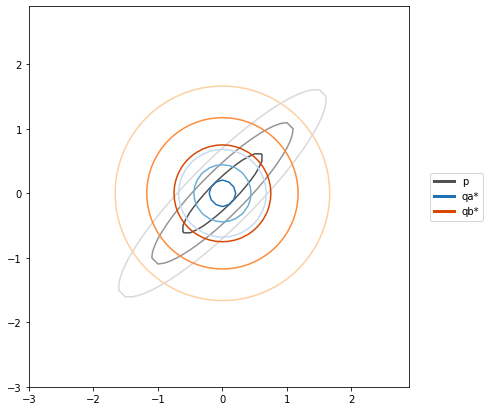
\includegraphics[width = 0.5\textwidth]{1c_contour_plot.png}
        \caption{Contour lines of true distribution $p ~ \cN(\mu, \Sigma)$,
                $q_a^\star$ which minimizes $\textrm{KL}(q||p)$ and exhibits mode-seeking behavior, and
                $q_b^\star$ which minimizes $\textrm{KL}(p||q)$ and exhibits mean-seeking/mass-covering behavior.}
    \end{figure}
\end{enumerate}



\clearpage

%%%%%%%%%%%%%%%%%%%%%%%%%%%%%%%%%%%%%%%%%%%%%%%%%
\textbf{Problem 2:}  \textit{Variational autoencoders (VAE's)} 

In class we derived VAE's as generative models~$p(x, z; \theta)$ of observations~$x \in \reals^P$ and latent variables~$z \in \reals^D$, with parameters~$\theta$.  We used variational expectation-maximization to learn the parameters~$\theta$ that maximize a lower bound on the marginal likelihood,
\begin{align*}
    \log p(x; \theta) \geq \sum_{n=1}^N \bbE_{q(z_n | x_n, \phi)}\left[\log p(x_n, z_n; \theta) - \log q(z_n \mid x_n, \phi) \right] \triangleq \cL(\theta, \phi).
\end{align*}
The difference between VAE's and regular variational expectation-maximization is that we constrained the variational distribution $q(z \mid x, \phi)$ to be a parametric function of the data; for example, we considered,
\begin{align*}
    q(z_n \mid x_n, \phi) &= \cN \left(z_n \mid \mu(x_n; \phi), \mathrm{diag}([\sigma_1^2(x_n; \phi), \ldots, \sigma_D^2(x_n; \phi)]) \right),
\end{align*}
where~$\mu: \reals^P \to \reals^D$ and $\sigma_d^2: \reals^P \to \reals_+$ are functions parameterized by~$\phi$ that take in a datapoint~$x_n$ and output means and variances of~$z_n$, respectively.  In practice, it is common to implement these functions with neural networks.  Here we will study VAE's in some special cases.  For further reference, see Kingma and Welling (2019), which is linked on the course website.

\begin{enumerate}[label=(\alph*)]
    \item Consider the linear Gaussian model factor model,
    \begin{align*}
        p(x_n, z_n; \theta) &= \cN(z_n; 0, I) \, \cN(x_n \mid A z_n, \, V),
    \end{align*}
    where~$A \in \reals^{P \times D}$, $V \in \reals^{P \times P}$ is a diagonal, positive definite matrix, and~$\theta = (A, V)$.  Solve for the true posterior~$p(z_n \mid x_n, \theta)$.
    
    \begin{solution}
    Following the marginal and conditional Gaussian distribution expressions as given in Bishop, Chapter 2.3 (p93), the true posterior is given by
    \begin{align*}
        p(z_n \given x_n) &= \cN(\Sigma\, A^\trans V^\inv x_n, \Sigma)
        \numberthis\label{2a_posterior}\\
        & \textrm{where } \Sigma = (I + A^\trans V^\inv A)^\inv
    \end{align*}
    \end{solution}
    
    \item  Consider the variational family of Gaussian densities with diagonal covariance, as described above, and assume that~$\mu(x; \phi)$ and $\log \sigma_d^2(x; \phi)$ are linear functions of~$x$.  Does this family contain the true posterior?  Find the member of this variational family that maximizes~$\cL(\theta, \phi)$ for fixed $\theta$. (Hint: use your answer to Problem 1a.)
    
    \begin{solution}
    This variational family contains the true posterior only if $A^\trans A$ is diagonal, or equivalently if the rows of $A$ are linearly independent/orthogonal to each other. Then, the covariance matrix of the posterior \eqref{2a_posterior} $\Sigma$ is also diagonal.

    We minimize the KL divergence between the true and approximate posteriors to find the member of $\cQ$ which maximizes the evidence lower bound:
    \begin{align*}
        q^\star = \arg\min_{q\in\cQ}\textrm{KL}(q(z_n\given x_n; \phi) || p(z_n \given x_n; \theta))
    \end{align*}
    Using the results from problem 1A, we have
    \begin{align*}
        \mu_\phi^\star &= \mu_\theta = (I + A^\trans V^\inv A)^\inv x_n \\
        \Sigma_\phi^\star &= \textrm{diag}\left[\Sigma_\theta^\inv\right]^\inv
        = \textrm{diag}\left[(I + A^\trans V^\inv A)\right]^\inv
    \end{align*}
    \end{solution}
    
    \item Now consider a simple nonlinear factor model,
    \begin{align*}
        p(x_n, z_n; \theta) &= \cN(z_n \mid 0, I) \, \prod_{p=1}^P \cN(x_{np} \mid e^{a_p^\trans z_n}, v_p),
    \end{align*}
    parameterized by~$a_p \in \reals^D$ and~$v_p \in \reals_+$.  The posterior is no longer Gaussian, since the mean of~$x_{np}$ is a nonlinear function of the latent variable.\footnote{For this particular model, the expectations in~$\cL(\theta, \phi)$ can still be computed in closed form using the fact that~$\bbE[e^z] = e^{\mu + \frac{1}{2}\sigma^2}$ for $z \sim \cN(\mu, \sigma^2)$.}  
    
    Generate a synthetic dataset by sampling $N=1000$ datapoints from a $D=1$, $P=2$ dimensional model with~$A = [1.2, 1]^\trans$ and~$v_p = 0.1$ for $p=1,2$.  Use the reparameterization trick and automatic differentiation to perform stochastic gradient descent on~$-\cL(\theta, \phi)$.
    
    Make the following plots: 
    \begin{itemize}
        \item A scatter plot of your simulated data (with equal axis limits).
        \item A plot of $\cL(\theta, \phi)$ as a function of SGD iteration. 
        \item A plot of the model parameters~$(A_{11}, A_{21}, v_1, v_2)$ as a function of SGD iteration.
        \item The approximate Gaussian posterior with mean $\mu(x; \phi)$ and variance~$\sigma_1^2(x; \phi)$ for $x \in \{(0, 0), (1, 1), (10, 7)\}$ using the learned parameters~$\phi$.
        \item The true posterior at those points. (Since $z$ is one dimensional, you can compute the true posterior with numerical integration.)
    \end{itemize}
    Comment on your results.
    
    \begin{solution}
    
    \begin{figure}
        \centering
        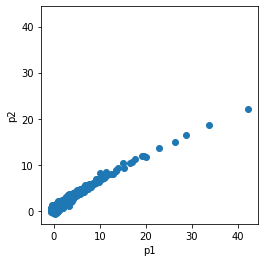
\includegraphics[width=0.4\textwidth]{2c_1_synthetic-data.png}
        \caption{Synthetic data}
    \end{figure}

    Both the encoder and the decoder are a neural network that parameterizes a Gaussian distribution (with diagonal covariance):

    \begin{align*}
        (\mbmu, \mbsigma^2) &=\textrm{ EncoderNeuralNet}_{\phi}(\mbx) \\
        q_{\phi}(\mathbf{z} \given \mbx) &=\cN(\mathbf{z} ; \mbmu, \textrm{diag}(\boldsymbol{\sigma^2})) \\
        & \\
        p(\mbz) &= \cN(\mbz; 0, \bbI) \\
        \textrm{p} &= \textrm{ DecoderNeuralNet}_{\theta}(\mbz)
    \end{align*}
The weights of each network is shared between their respective means and covariances. To ensure that a valid covariance is outputted, the last layer of the covariance pipe is a SoftPlus function.

The ELBO was then calculated using the reparameterization trick, by introducing a new random variable $\epsilon\sim\cN(0,I)$ to take the stochasticity out of the $z$ variable.

\begin{align*}
    \epsilon &\sim \cN(0,\bbI) \\
    \mu_\phi, \sigma_\phi^2 &\leftarrow \textrm{ EncoderNN } \\
    z &= \mu + \sqrt{\sigma^2}*\epsilon) \\
    \log q &= \sum_p \log \cN(z \given \mu, \sigma^2) \\
    & \\
    \mu_\theta, \sigma_\theta^2 &\leftarrow \textrm{ DecoderNN } \\
    \log p &= \sum_p \log \cN(z \given 0, \bbI) + \log \cN(\textrm{batch} \given \mu_\theta, \sigma_\theta^2)
    & \\
    \cL(\theta, \phi) &= \frac{1}{N}\sum_n \log p - \log q
\end{align*}
\begin{figure}
    \centering
    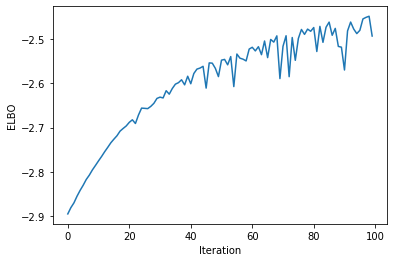
\includegraphics[width=0.4\textwidth]{2c_2_elbo.png}
    \caption{ELBO as function of SGD iteration}
\end{figure}

I was unable to figure out how to save intermediate values of the means and variances through iteration, since they are Traced objects and therefore abstracted. Associated code can be found in the colab notebook (link in the comments section of the upload, I was having trouble exporting it as a PDF due to Latex compiltion issues and my write-up is not letting me write the link down verbatim).

\end{solution}
\end{enumerate}

\clearpage

%%%%%%%%%%%%%%%%%%%%%%%%%%%%%%%%%%%%%%%%%%%%%%%%%
\textbf{Problem 3:} \textit{Semi-Markov models}

Consider a Markov model as described in class and in, for example, Chapter 13 of \textit{Pattern Recogntion and Machine Learning} by Bishop,
\begin{align*}
    p(z_{1:T} \mid \pi, A) &= p(z_1 \mid \pi) \prod_{t=2}^T p(z_t \mid z_{t-1}, A),
\end{align*}
where~$z_t \in \{1, \ldots, K\}$ denotes the ``state,'' and
\begin{align*}
    p(z_1 = i) &= \pi_i \\
    p(z_t = j \mid z_{t-1} = i, A) &= A_{ij}.
\end{align*}
We will study the distribution of state durations---the length of time spent in a state before transitioning.  Let $d \geq 1$ denote the number of time steps before a transition out of state $z_1$.  That is, $z_1 = i, \ldots, z_{d}=i$ for some~$i$, but $z_{d+1} \neq i$.

\begin{enumerate}[label=(\alph*)]
    \item Show that $p(d \mid z_1=i, A) = \mathrm{Geom}(d \mid p_i)$, the probability mass function of the geometric distribution.  Solve for the parameter~$p_i$ as a function of the transition matrix~$A$.
    
    \begin{solution}
    \begin{align*}
        p(d\given z_1=i, A) &= p(\{z_t=i\}_{t=1}^d, z_{d+1}\neq i \given z_1 =i,\, A) \\
            &= p(z_{d+1}\neq i \given z_d=i, A)\, p(\{z_t=i\}_{t=1}^d \given z_1 =i,\, A) \\
            &= p(z_{d+1}\neq i \given z_d=i, A)\,  p(z_t =i \given z_{t-1} =i,\, A) \\
            &= (1-A_{ii})\,A_{ii}^{d-1} = \textrm{Geom}(d-1 \given 1-A_{ii})
    \end{align*}
    so the parameter $p_i = 1-A_{ii}$, i.e. the probability of transitioning to another state.
    \end{solution}
    
    \item We can equivalently represent $z_{1:T}$ as a set of states and durations~$\{(\tilde{z}_n, d_n)\}_{n=1}^N$, where $\tilde{z}_n \in \{1, \ldots, K\} \setminus \{\tilde{z}_{n-1}\}$ denotes the index of the $n$-th visited state and $d_n \in \naturals$ denotes the duration spent in that state before transition.  There is a one-to-one mapping between states/durations and the original state sequence:
    \begin{align*}
        (z_1, \ldots, z_T) &= (\underbrace{\tilde{z}_1, \ldots, \tilde{z}_1}_{d_1\,\mathrm{times}}, \underbrace{\tilde{z}_2, \ldots, \tilde{z}_2}_{d_2\,\mathrm{times}}, \ldots \underbrace{\tilde{z}_N, \ldots, \tilde{z}_N}_{d_N\,\mathrm{times}}).
    \end{align*}
    Show that the probability mass function of the states and durations is of the form
    \begin{align*}
        p(\{(\tilde{z}_n, d_n)\}_{n=1}^N) &= p(\tilde{z}_1 \mid \pi) \left[ \prod_{n=1}^{N-1} p(d_n \mid \tilde{z}_n, A) \, p(\tilde{z}_{n+1} \mid \tilde{z}_n, A) \right] p(d_N \mid \tilde{z}_N, A),
    \end{align*}
    and derive each conditional probability mass function.
    
    \begin{solution}
    The durations of each state is only conditionally dependent on the state itsel, and the next state is only conditionally dependent on its immediately preceding state. This Markov/duration model provides us with strong structures to simplify the joint distribution as follows:
    \begin{align*}
        p(\{(\tilde{z}_n, d_n)\}_{n=1}^N)
            &= p(\tilde{z}_1\given\pi)\,p(d_1 \given \tilde{z}_1,\,A)\,
                p(\tilde{z}_2\given \tilde{z}_1,\,A)\,p(d_2 \given \tilde{z}_2,\,A)\,
                \ldots p(d_N \given \tilde{z}_{N}, \,A) \\
            &= p(\tilde{z}_1 \mid \pi) \left[ \prod_{n=1}^{N-1} p(d_n \mid \tilde{z}_n, A) \, p(\tilde{z}_{n+1} \mid \tilde{z}_n, A) \right] p(d_N \mid \tilde{z}_N, A)
    \end{align*}
    Then, the conditional PMF of each term is
    \begin{align*}
        p(\tilde{z}_1 \mid \pi)
            &= p(z_1 = \tilde{z}_1 \given \pi) = \pi_{\tilde{z}_1}
            && \\
        p(\tilde{z}_{n+1} \mid \tilde{z}_n,\, A)
            &= A_{\tilde{z}_{n+1}\tilde{z}_{n}}
            &&\quad \textrm{for } n=1,\ldots,N-1 \\
        p(d_n \mid \tilde{z}_n,\, A)
            &= \textrm{Geom}(d_n-1\given p_{\tilde{z}_{n}})
            &&\quad \textrm{for } p_{\tilde{z}_{n}}=A_{\tilde{z}_{n}\tilde{z}_{n}}, n=1,\ldots,N
    \end{align*}
    \end{solution}
    
    \item \emph{Semi-Markov} models replace $p(d_n \mid \tilde{z}_n)$ with a more flexible duration distribution.  For example, consider the model,
    \begin{align*}
        p(d_n \mid \tilde{z}_n) &= \mathrm{NB}(d_n \mid r, \theta_{\tilde{z}_n}),
    \end{align*}
    where $r \in \naturals$ and $\theta_k \in [0, 1]$ for $k=1,\ldots,K$.  Recall from Assignment 1 that the negative binomial distribution with integer~$r$ is equivalent to a sum of~$r$ geometric random variables.  Use this equivalence to write the semi-Markov model with negative binomial durations as a Markov model on an extended set of states~$s_n \in \{1, \ldots, Kr\}$.  Specifically, write the transition matrix for $p(s_n \mid s_{n-1})$ and the mapping from $s_n$ to $z_n$.
    
    \begin{solution}
    Let us index the states by $m$, so that there are a total of $M = Kr$ states in the extended set.
    This model is called semi-Markovian because for every new state $\tilde{z}_n$ that it enters,
    it must then sequentially visit every $r$ associated state (non-Markov process)
    before it can transition to a different state $\tilde{z}_{n+1}$ (Markovian).
    
    As an example, suppose $K = 4$ and $R = 2$, then our sets look like
    \begin{align*}
        \tilde{z} &= \{1, 2, 3, 4\} \\
        s &= \{1_1,1_2,2_1,2_2, 3_1, 3_2, 4_1, 4_2\} = {1, 2, 3, 4, 5, 6, 7, 8}
    \end{align*}
    When we enter $\tilde{z}_n=1$ for example, $s_m = 1_1$ and $s_{m+1}=1_2$ before it can transition to any other $\tilde{z}_{n+1}\neq\tilde{z}_{n}$. 
    Then, let the map from $s_m$ to $\tilde{z}_n$ be defined by $M(s_m) = \lceil s_m/r \rceil$.
    We also define the boolean functions identifying if a state is a entry/beginning state ($B(s_m) = [s_m\% R == 1]$) or a terminal state $T(s_m) = [s_m\% R == 0]$. Therefore,
    \begin{align*}
        p(s_m \given s_{m-1}) = \begin{cases}
                \theta_{\tilde{z}_n} & \textrm{if } M(s_{m-1}) == M(s_m)\\
                A_{\tilde{z}_{n+1}{\tilde{z}_n}}
                    & \textrm{if } M(s_{m-1})\, != M(s_m),\, T(s_{m-1})\, \textrm{and } B(s_m)\\
                0   & \textrm{otherwise}
            \end{cases}
    \end{align*}

    \end{solution}
    
\end{enumerate}


\end{document}